\documentclass[11pt,a4paper]{article}

\usepackage{jheppub}
\usepackage{fontspec-luatex}
\usepackage{dsfont}
\usepackage{nicefrac}
\usepackage{bm}
\usepackage{mathsettings}
\usepackage{xparse}
\usepackage{mathrsfs}
\usepackage[none]{hyphenat}
\usepackage{tabularx}
\usepackage{makecell}
\usepackage{empheq}
\usepackage{pifont}
\usepackage{hhline}
\usepackage{tikz}
\usepackage[
backend=biber,
style=numeric,
sorting=none
]{biblatex}

\addbibresource{bibliography.bib}

\graphicspath{{./figures/}}

\usetikzlibrary{ext.paths.ortho,  % -|- and |-| path operations
	quotes,
	tikzmark,
}
\tikzset{
	is/.style = {inner ysep=2pt},
	lbl/.style = {anchor=#1, inner sep=1pt, align=center,
		font=\footnotesize\linespread{0.84}\selectfont},
	lbl/.default=south
}


\newcommand{\bfnt}[1]{{\bfseries #1}}
\newcommand{\ifnt}[1]{{\itshape #1}}

% https://tex.stackexchange.com/a/531829/200495
\makeatletter
\gdef\@fpheader{}
\makeatother

% Package siunitx has deprecated Angstrom.
% https://tex.stackexchange.com/q/610292/200495
\DeclareSIUnit\angstrom{\text{\AA}}

% https://tex.stackexchange.com/a/65934/200495
\newcommand\Tstrut{\rule{0pt}{2.6ex}}       % top strut
\newcommand\Bstrut{\rule[-1.1ex]{0pt}{0pt}} % bottom strut

% Courtsey: https://tex.stackexchange.com/a/326380/200495
% Syntax: \colorboxed[<color model>]{<color specification>}{<math formula>}
\makeatletter
\newcommand*{\colorboxed}{}
\def\colorboxed#1#{%
	\@colorboxed{#1}%
}
\newcommand*{\@colorboxed}[3]{%
	% #1: optional argument for color model
	% #2: color specification
	% #3: formula
	\begingroup
	\colorlet{cb@saved}{.}%
	\color#1{#2}%
	\boxed{%
		\color{cb@saved}%
		#3%
	}%
	\endgroup
}
\makeatother

% Provides \Acolorboxed[color]{equation with align character (&)}. 
% Colored variant of \Acolorboxed{} from mathtools package.
% Courtsey:https://tex.stackexchange.com/a/610299/200495
\makeatletter
\newcommand*\Acolorboxed[2][red]{%
	\let\bgroup{\romannumeral-`}%
	\@Acolorboxed{#1}#2&&\ENDDNE
}
\def\@Acolorboxed#1#2&#3&#4\ENDDNE{%
	\ifnum0=`{}\fi
	\setbox\z@\hbox{$\displaystyle#2{}\m@th$\kern\fboxsep \kern\fboxrule}%
	\edef\@tempa{\kern\wd\z@ & \kern-\the\wd\z@ \fboxsep\the\fboxsep \fboxrule\the\fboxrule}%
	\@tempa
	\fcolorbox{#1}{white}{\m@th$\displaystyle#2#3$}%
} 
\makeatother


\begin{document}
	
	\title{A Brief Primer on Thermionic Emission}
	\author{Muhammad Nasim}
	\affiliation{Semester VI, B.Sc. Physics (Hons.)\\Dept. of Physics, Scottish Church College\\University of Calcutta, India.}
	\date{\today}
	
	\maketitle
	\flushbottom
	
	\newpage
	
	\section{A. Scope and objectives.}
	
	\subsection{Definitions.}
	The emission of electrons across the boundary surface that
	separates a heated electronic conductor from an otherwise nonconducting space
	has become synonymous with the term ``thermionic emission". The broadest
	application of the word thermionic might include the emission of charged atomic
	or molecular particles that may carry with them either a net positive or a net
	negative charge. Since these phenomena are so very different basically, this
	article will be devoted exclusively to the more fundamental aspects of the
	experimental and the theoretical investigations of the phenomenon of electron
	emission from heated conductors.
	
	Thousands of experiments have been reported in the literature and serve
	as the basic work material from which an explanation of the phenomenon in
	terms of the fundamental principles of physics emerges. The studies relate to
	four surface classifications which are:
	
	\begin{itemize}
		
		\item clean homogeneous surfaces;
	
		\item clean heterogeneous surfaces;
		
		\item simple composite surfaces;
		
		\item complex surfaces.
		
	\end{itemize}
	
	To clarify these classifications an illustration of each will be given. Single
	crystal wires of circular cross section have been used as sources of thermionic
	electrons and provide the nearest approach to the realization of experimental
	conditions appropriate to theoretical interpretation.
	
	Emission can be observed and investigated in detail from the more important crystallogr-\ aphically homogeneous surfaces. These surfaces must be maintained
	under such perfect vacuum conditions that an absolutely negligible fraction of
	a monomolecular layer of impurity is present. Since fundamental studies show
	that the thermionic emission is dependent not only on the atomic composition
	of the emitting conductor but also on the crystallographic structure of the exposed surfaces, it is evident that practically all investigations that describe the
	electron emission from polycrystalline substances yield data characteristic only
	of the particular specimen. In general such observations measure the electron
	emission summed over an assembly of \emph{heterogeneous surfaces}, which can never
	be accurately described. Most of the work reported in the literature of the subject applies to these surfaces.
%------------------------	
	
	At a given temperature, the efficiency of electron emission from a given
	conductor may be altered through many orders of magnitude by the adsorption
	of polarizable atoms or molecules on an otherwise clean homogeneous or heterogeneous underlying conductor. The presence of a surface-layer coverage having a
	density even smaller than 1/100 part of a monolayer can be observed to alter the
	emission properties. Such surfaces are classified as \emph{simple composite surfaces} if the extent of the coverage is of the order of a monolayer or less.
	
	%--------------------
	The last of the above four classifications, the \emph{complex surface}, is by far the
	most important in terms of its usefulness as a source of electrons and includes
	as its most important member the \emph{oxide cathode}. The structure represents an
	emitter which depends on the conduction of a heated metallic support such as
	nickel or platinum upon which has been placed, after due processing, a layer of
	alkaline earth oxide crystals. The surfaces of these crystals serve as the emitting
	areas. These crystals are generally solid solutions of barium oxide and strontium
	oxide of comparable proportions and sometimes have traces of other substances
	added. It is not unexpected that such a complex emitter will have properties very
	difficult to explain.
	
	\subsection{Theory and experiment.}
	
	It is an illusion to believe that the main features
	of thermionic emission have been worked out theoretically and are in agreement
	with experiment.  In spite of the generality often associated with the thermodynamic interpretation of thermionic emission, emphasis must be given to the
	fact that this branch of theory cannot be relied upon to give accurate information
	concerning the current flow across a boundary under experimental conditions
	that violate the basic assumptions of the theory. The most important assumption
	made is that the system under consideration can be bounded in a manner
	that will still permit the actual measurement of an electron emission across a
	boundary. Thermodynamic considerations can be applied to the electron gas
	in the interior of a single crystal of conducting substance so cut out as to bound
	the interior cavity by surfaces of perfect homogeneity as regards their crystal
	structure. With the combined help of the equations of thermodynamics and
	electrostatics the time average of the density of electrons can be specified as a
	function of the coordinates within the cavity. The pressure that these electrons
	would exert on the surface of the cavity can be computed with confidence and
	from these quantities one might presume to calculate a current of electrons which
	would flow from the interior of the conducting specimen across a surface boundary to the region just outside the conductor. To assume that such a calculation
	of the current would be directly related to an observable emission current is
	wrong. No theory as general as this can predict the fraction of the electrons
	which are reflected at the boundary.
	
	Even though usually considered to be less general, the statistical theory of
	an assembly of free electrons is more capable of giving valid information concerning the thermionic emission process. It will therfore be appropriate to base
	practically all of the theoretical analysis brought forward in this chapter on the
	application of the statistics of free electrons to thermionic emission phenomena.
	
	
	\section{B. Historical highlights.}
	
	\subsection{Introduction.}
	
	It will be the purpose of this section to review briefly some
	of the main events that have marked both the development of the theory and
	the understanding of thermionic emission as well as the technological advances
	which have been made during the past 70 years. Following this qualitative
	review of events a detailed analysis will be given to review the present state of
	our understanding with respect both to theory and experiment.
	
	\subsection{Discovery and identification of thermionic emission.}
	
	That negative electricity escapes from hot filaments was probably first established by THOMAS A.
	EDISON and later identified by WILLIAM H. PREECE as the ``EDISON Effect".
	The account by PREECE of his own experiments on the EDISON effect does not
	separate the phenomenon now recognized as thermionic emission from the
	``blue effect" which was evidently the ionization of the residual gas produced
	by the electrons as they were accelerated from the negative hot filament to the
	plate of the diode. The identification of the charge carrier emitted from the hot
	carbon filament as a particle with a very small mass compared with that of a
	hydrogen ion and with a charge equal in magnitude but opposite in sign to that
	of the hydrogen ion was made by J. J. THOMSON. In spite of the important
	experiments of J. J. THOMSON, general agreement that electron flow through
	conductors and electron emission from hot surfaces are truly different phenomena from ionic flow through substances and ionic conduction through gases did not
	come until about 1914.
	
	\subsection{RICHARDSON equations.}
	
	Thermionic emission is so intimately associated
	with the phenomenon of electronic conducti- \ on in solids that advances in these
	two fields of scientific investigation are associated. The DRUDE development
	of the theory of free electrons in metallic conductors paved the way for the
	better understanding of thermionic emission which marked the contributions
	of. W. RICHARDSON. The basic idea of work-function as being a measure of
	the energy per electron required to transfer charges from the interior of the
	conductor to the field-free space outside of it is largely due to RICHARDSON.
	Founded on a very literal classical interpretation of the free electron theory
	of electronic conduction in metals, RICHARDSON derived his first thermionic
	emission equation which took the following form:
	
	\begin{equation}
		I = ne (\frac{k}{2 \pi m})^\frac{1}{2} T^\frac{1}{2} e^\frac{- e \phi}{k T}
	\end{equation}

The recognition of difficulties encountered by the classical free electron theory
of conduction and its relation to the specific heat of metals led RICHARDSON
and VON LAUE to the ``$T^2$ " equation given as follows:

	\begin{equation}
		I = A T^2 e^\frac{- e \phi}{k T}
	\end{equation}

	In its original form this equation depended upon thermodynamic arguments and
	at the present time it is accepted as the correct expression for electron current
	flow at a boundary which is in a system maintained under conditions of thermodynamic equilibrium. The mistake generally made in the application of this
	equation is that the current I is identified as the thermionic emission current one
	should expect to observe in a laboratory experiment. The current density of
	Eq.(2.1) is independent of reflection and of other phenomena that may alter
	the distribution in energy of the electrons which do cross the boundary in an
	actual emission experiment. A second common error in the application of Eq.(2.2)
	to thermionic emission is the assumption that the true work-function $\phi$ is a constant.
	
	\subsection{CHILD-LANGMUIR space charge.}
	
	A second effect produced by accelerating
	fields-an important one in the understanding of thermionic emission-was
	recognized by LANGMUIR and CHILD and others as being accounted for by the
	phenomenon of space charge.
	
	As the temperature of an emitting conductor increases, the observed current
	does not increase indefinitely, even though a fixed strongly accelerating positive
	potential is maintained on the electron collector. If the number of electrons in
	transit between the emitter and the collector exactly equals the total surface
	charge maintained on the collector by the external circuit, then the electric field
	at the emitter becomes zero. Further increases in temperature are followed by
	very little increase in observed current because of the development of a retarding
	field at the surface of the emitter produced by space-charge. Even though
	space-charge effects are strongly dependent on electrode geometry and act in
	the space well outside of the thermionic emitter itself, it is necessary to have a
	full understanding of their influence. Thermionic emission is an electron flow
	observed as a current between suitably placed electrodes and the phenomenon
	of space charge seldom should be neglected in the interpretation of the observations
	
	\section{C. Theory.}
	
	\subsection{Free electrons.}
	
	The basic concepts needed for the derivation of thermionic
	emission equations are very elementary and yet they are sufficient for the
	purpose. One pictures the interior of a conducting crystal as an organized arrangement of atoms characterized by specific interatom- \ ic distances which are specifically dependent on the atomic composition and the phase taken on by the crystal,
	depending upon the temperature and the previous temperature history of the
	specimen. Each crystal as a whole should be thought of as being electrically
	neutral within any extended region in the interior. Any excess of charge either
	positive or negative will be found at the surface only. Quantum theory indicates
	that most of the electrons that neutralize the positive charge on the atomic
	nuclei are localized near them and in general contribute nothing to the electrical
	conductivity of the specimen. The valence electrons associated with these
	atoms, however, occupy quantum states that extend throughout the entire interior of each isolated crystal and it is to these electrons that the statistical
	theory of the free electron gas may be applied. The free electron theory as applied
	to these valence electrons describes their behavior in practically classical terms
	and finally depends upon experiment to justify the applicability of the simplifying assumptions. It is the purpose of this article to indicate as clearly as possible
	that the most recent experiments serve to support strongly the concepts of the
	mechanism of thermionic emission which can be derived from the theory even
	though they are based on a semiclassical analysis of behavior of valence electrons
	in a conductor.
	
	\subsection{Three basic assumptions.}
	
	The first assumption made for the development of this theory is that the inter-electronic forces can be neglected and therefore the electrons behave as though they were particles of three degrees of freedom.
	The phase space suitable for representing the behavior of an assembly of electrons
	can therefore be taken to be a six-dimensional phase space in which a representative point exists for each electron in the assembly. The six bits of information
	needed to localize this representative point are three coordinates and three
	components of momentum. The second assumption is that for each quantum
	state an extension in phase space of size $h^3$ is needed and that a representative
	point cannot be localized (nor need it be) more specifically than to indicate
	that one representative point lies within the quantum-state region. Actually
	this is not quite the whole story because quantum principles permit two electrons
	to occupy a single quantum state if their spin vectors are always antiparallel.
	A factor 2 that appears repeatedly in the equations derived on these assumptions
	is therefore this weight factor which is thus incorporated into the theory.
	Already the third postulate has been mentioned, namely, the PAULI Exclusion
	Principle, which limits the number of electrons in a given quantum state to two
	with antiparallel spin vectors.
	
	It is the purpose of a statistical theory to find an expression for the distribution of representative points in phase space which is consistent with basic principles of thermodyna- \ mics and has associated with it the greatest likelihood of
	occurrence. The function thus obtained, without the need for introducing any
	additional assumptions, is the following:
	
	\begin{equation}
		f( \epsilon ) ~ dx~dy~dz~dp_x ~ dp_y ~ dp_z = 2 \frac{dx ~ dy ~ dz ~ dp_x  ~ dp_y ~ dp_z}{h^3} [ \frac{1}{e^\frac{\epsilon - \mu}{kt} + 1}]
	\end{equation}
	
	Some explanation of this equation may make its use and meaning easier to grasp.
	The energy is generally separable into two terms, one of which expresses the
	kinetic energy of a particle whose representative point lies in a specified region
	in phase space, and the other term is the potential energy expressible in terms of
	the coordinates of a particle whose representative point is in that region in phase
	space. The quantity $\mu$ is a constant for a given problem which contains implicitly
	the concentration of electrons and is a function of the temperature. The fundamental concept that determines the value of this parameter is that the integration
	of Eq.(3.1) over the entire phase space shall exactly equal the number of electrons in the assembly, that is, the number of free electrons within a crystal, for
	example. Although this statement defines the manner in which the constant $\mu$ 
	is determined, there is a second meaning to the constant which is interesting to
	note, if it applies to a concentration of electrons of the order of $10^{20}$ per $cm^3$. The energy value $\mu$  is that to be associated with that quantum state for which
	the probability of occupancy is exactly one-half.
	
	For electron concentrations less than approximately $10^{19}$ per $cm^3$ the appropriate value of $\mu$  is generally a negative number. This statement demands a
	word of explanation. The simplest application of Eq.(3.1) is made to regions
	in coordinate space over which there is no change in potential energy. It is
	therefore sufficient for the present purpose to apply Eq.(3.1) to problems in
	which the potential energy may be taken to be zero. In that case the energy $\epsilon$ 
	will be the kinetic energy of the electron whose representative point lies in a
	particular region of phase space. In problems of this kind which occur in connection with the theory of the oxide cathode, the algebraic sign of the quantity $\mu$ 
	can be defined as negative, and therefore, it lies below the conduction band in
	the energy, band system. All of the available quantum states associated with
	the particular problem for low-density distributions of the electrons are less
	than half filled if $\mu$  is negative.
	
	Note that the extension in phase space $2 \frac{dx ~ dy ~ dz ~ dp_x  ~ dp_y ~ dp_z}{h^3}$ represents
	the number of quantum states in this extension, since the extension per quantum
	state is $h^3$
	, as mentioned previously. The factor 2 is the double occupancy of a
	quantum state by the two electrons with antiparallel spin vectors.
	
	
	Finally, the factor in the square brackets of Eq.(3.1) can be identified by
	its name the ``FERMI factor" which gives a direct means of computing the
	probability that a given quantum state identified by its energy e will be occupied.
	The energy is given explicitly in terms of the momenta and the coordinate values
	associated with the representative point in phase space. The name given to
	the quantity $\mu$  is the ``FERMI level". It is evident at once that if the numerical
	value of $\mu$  is positive, then there can be an energy level $\epsilon$ exactly equal to $\mu$  and,
	as mentioned above, the FERMI factor takes on the value $\frac{1}{2}$.
	
	\subsection{The electron flow equation.}
	
	Although Eq.(3.1) is the basic starting point for all equations relevant to thermionic emission, the following equation which is derived directly from Eq.(3.1) without the introduc-\ tion of any approximations is the most important equation applicable to thermionic emission.
	
	\begin{equation}
		N(\epsilon_x)d\epsilon_x = 2 \frac{2 \pi m k T}{h^3} ln(1+e^{-\frac{\epsilon_x- \mu}{k T}}) d\epsilon_x
	\end{equation}
	
	The independent variable in this equation $\epsilon_x$ is defined by
	\begin{equation}
		\epsilon_x = \frac{p_x^2}{2m}
	\end{equation}
	
	By the use of Eq.(3.2), the number of electrons $N(\epsilon_x)d\epsilon_x$ that cross a unit area in unit time with kinetic energy associated with the positive $x$ direction of motion can be computed for the energy range, $d\epsilon_x$. This equation holds for all values of $\mu$, either positive or negative, and therefore applies to all densities of electrons provided $\mu$ is expressed relative to the energy level for which the kinetic energy is zero or, in other words, with respect to the potential energy at the region in space for which the number of electrons crossing a boundary perpendicular to the $x$ direction is being computed. The first application of this formula will be to compute the ``random" currents which impinge on various boundaries of a pillbox-like cavity within the interior of a homogeneous crystal.
	
	\subsection{Electrons in a cavity.}
	
	The pillbox problem is of interest because it is the
	only example of the application of theory to an experimentally realizable structure
	for which all of the essential details are easy to describe. The structure visualized
	is shown in Fig. 1. The cross-hatched solid structure S represents a section
	through the interior of a single crystal and the cavity within this crystal is represented by $C$.
	
	The perpendicular distance across that cavity, $a$, $ b$, should be visualized as
	being not less than $10^{-4} cm $. and can very well be any amount larger than this.
	The requirement that the cavity be essentially pillbox form is necessary because
	of the need to have the entire interior of the cavity of a single surface structure
	type. The pillbox has the further advantage that the problem can be handled
	exactly, even though sufficient electrons exist in the cavity to give an appreciable space-charge field there. The first steps of the discussion can be carried
	through without the introduction of space charge as a factor of any importance.
	
	In the energy diagram of Fig. 2 the potential' energy of an electron is shown
	as a function of distance as one progresses in the $x$ direction from $A$ to $B$. The region $A$ to $a$, is the potential in the interior of the solid taken here to be uniform.
	It will be shown later that the periodicity of the true potential is of no consequence in the thermionic emission theory. The potential of the electron in the
	space between a and b is shown to be higher than that in the interior of the metal
	by an amount $W_a$. This energy difference is the integration of all of the actual
	forces that act on an electron as it escapes from the metal into the cavity. In
	the absence of space charge the cavity potential will be constant at distances
	greater than approximately $10^{-5}$ cm. from either surface, since the dominant
	long-range force acting on an electron is the mirror-image force which at this
	distance has fallen to a negligible amount. Eq.(3.2) may be used to calculate
	the number of electrons which approach the boundary from the left at a, with
	energy between $\epsilon_x$ and $\epsilon_x$ $ + d\epsilon_x$ associated with the $x$ component of the momentum. In the space between a and b the corresponding energy state lies at $\epsilon_x^{'}$.
	
	%%%%%%%%%%%%%%%%%%%%%%%%%%%%%%%%%%%%%%%%%%%%%%%%%%%%%%%%%
	
	
	\begin{figure}[h]
		\centering
		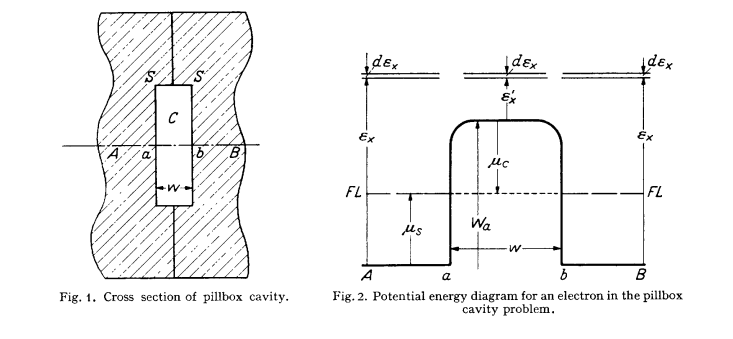
\includegraphics[width=\textwidth]{fig1.png}
	\end{figure}
	
	
	%%%%%%%%%%%%%%%%%%%%%%%%%%%%%%%%%%%%%%%%%%%%%%%%%%%%%%%%%
	
	For the net current to be zero it is necessary that the current in this band from
	the left be equal and opposite to the current in the band which approaches surface a from the right. This statement would in general not be true if it were
	applied to a geometrical configuration in which currents were being observed
	as electron emission currents in the usual way. An essential part of this analysis
	is that the entire region surrounding the cavity be at a constant temperature
	and of course this includes the cavity itself.
	
	In the interior of the crystal the FERMI level, FL, is located at an energy $\mu_s$
	positive with respect to the potential energy line $Aa$ relative to which the kinetic
	energy $\epsilon_x$, is referred. The application of Eq.(3.2) shows that there is a simple
	and yet a necessary condition which must be satisfied if the cavity currents are
	in statistical equilibrium with the currents flowing in the solid. This condition
	is that the FERMI level be continuous right through the cavity space. Relative
	to the potential energy of an electron in the cavity, the FERMI level is negative,
	the amount shown as $\mu_c$. The formal writing of the two equations for the two
	electron streams serves to illustrate this point and will be used for further development. These equations are the following:
	
	\begin{equation}
		N_{xs}d\epsilon_x = 2 \frac{2 \pi m k T}{h^3} ln(1+e^{-\frac{\epsilon_x- \mu_s}{k T}}) d\epsilon_x
	\end{equation}
	
	\begin{equation}
		N_{xc}d\epsilon_x = 2 \frac{2 \pi m k T}{h^3} ln(1+e^{-\frac{\epsilon_x^{'}- \mu_c}{k T}}) d\epsilon_x
	\end{equation}
	
	It is clear from an inspection of these two equations that the necessary condition for the equality of these two flows of electrons is that the exponents be
	equal and the following equation may therefore be written:
	
	\begin{equation}
		\epsilon_x- \mu_s = \epsilon_x^{'}- \mu_c
	\end{equation}
	
	Eq. (3.7) gives additional relations as a result of the reorganization of Eq. (3.6)
	which are self-evident:
	
	\begin{equation}
		\epsilon_x- \mu_s = \epsilon_x^{'}- \mu_c = W_a
	\end{equation}
	
	The final rearrangement of this equation is written as follows:
	
	\begin{equation}
		-\mu_c = W_a - \mu_s = (true ~~ workfunction) \cross e = \phi e
	\end{equation}
	
	This equation stated in words demonstrates the fact that the true work-function
	expressed in energy units is a direct measure of the location of the FERMI level
	appropriate to the cavity space outside of a thermionic emitting conductor \emph{
	when equilibrium exists between the conductor and the space.}
	
	\subsection{The RICHARDSON equation.}
	
	The integration of Eq.(3.4) between the
	limits of $\epsilon_x$  = $W_a$ and $\infty$ gives a means of calculating the total electron current
	that impinges on the boundary at $a$ from the interior with the energy range limited, in such a way that any of the electrons included could have gone into the
	space if reflection effects at the boundary a did not exist. This result is given
	as Eq. (3.9). The integration of Eq. (3.5) gives the total current which would
	flow into the conductor from the exterior under conditions of perfect equilibrium.
	These two currents must be equal. These equations integrated give the following results:
	
	\begin{equation}
		I_s = \frac{2e(2\pi m kT)k T}{h^3} e^{-\frac{W_a - \mu_s}{kT}}
	\end{equation}
	
	\begin{equation}
	I_c = \frac{2e(2\pi m kT)k T}{h^3} e^{-\frac{\mu_c}{kT}}
	\end{equation}	
	
	The validity of Eq.(3.10) depends on the assumption that the numerical value
	of $\mu_c$ is not less than 5 $kT$ for an accuracy of better than $1\%$. For smaller values of $\mu_c$, other terms in the power series expansion must be used.
	
	The fact that $\mu_c$, is clearly a negative number implies that the electron density
	in the cavity space is smaller than approximately $10^{19}$ per $cm^3$ . Under these
	conditions the statistical theory gives a suitable expression for $\mu_c$ which is the
	following:
	
	\begin{equation}
		\mu_c = - kT ln[\frac{2(2\pi mkT)^{\frac{3}{2}}}{n_c h^3}]
	\end{equation}
	
	The substitution of this value for $\mu_c$, into Eq.(3.10) yields the following:
	
	\begin{equation}
		I_c = n_c e (\frac{kT}{2 \pi m})^{\frac{1}{2}}		
	\end{equation}
	
	in which $n_c$ is the concentration of electrons in the cavity space near enough to
	the surface so that space-charge fields can be neglected and yet far enough from
	the surface so that the mirror-image fields are negligible. This equation is the
	familiar one from classical mechanics and may be explained in the following
	terms: $(n_c/2)$ represents the concentration of electrons moving with a component
	of velocity in any specified direction; $2 (k T/2 \pi m)^{1/2}$ represents the average of the
	velocity component of these electrons in a classical distribution; and $e$ is the charge
	on an electron.
	
	The rewriting of Eq.(3.9) yields at once the RICHARDSON form of the equation so often misused when it is identified with observable thermionic emission.
	
	\begin{equation}
		I_s = \frac{4\pi m k^2 e}{h^3} T^2 e^{-\frac{W_a - \mu_s}{kT}}
	\end{equation}

	The first factor of this equation may be recognized as the familiar universal
	thermionic constant $A$.
	
	\begin{equation}
		A = \frac{4\pi m k^2 e}{h^3} = 120 ~~ amp/cm^2~T^2
	\end{equation}
	
	
	\medskip
	
	%\bibliographystyle{plain}
	%\bibliography{bibliography}
	\printbibliography
	
	
\end{document}